\documentclass{beamer}
\usepackage{amsmath, amsthm, amssymb, amsfonts, dsfont, mathrsfs, dirtytalk, tikz-cd, adjustbox, url, nicefrac, booktabs,array, graphicx,longtable, tabu,bm,cite,hyperref, comment, subcaption,multicol}



%%%%Macros
\newcommand{\e}{\epsilon}
\newcommand{\f}{\forall}
\newcommand{\R}{\mathbb R}
\newcommand{\st}{\text{ s.t. }}
\newcommand{\ex}{\exists}
\newcommand{\p}{\mathbb P}
\newcommand{\D}{\mathcal D(\Omega)}
\newcommand{\N}{\mathbb N}
\newcommand{\oo}{\Omega}
\newcommand{\harpoon}{\rightharpoondown}
\newcommand{\E}{\mathbb E}
\newcommand{\B}{\mathcal B}
\newcommand{\M}{\mathcal M}
\renewcommand{\H}{\operatorname{H}}
\newcommand{\dkl}{\operatorname{D_{K L}}}
\renewcommand{\d}{\: \mathrm{d}}
\newcommand{\id}{\operatorname{I d}}
\newcommand{\pspace}{(\oo, \Sigma, (\Sigma_t)_{t\geq 0}, \p)}

%%%%Theorem environments%%%%
\newtheorem{proposition}[theorem]{Proposition}
\newtheorem{remark}[theorem]{Remark}
\newtheorem{question}[theorem]{Question}
\newtheorem{idea}[theorem]{Idea}
\newtheorem{conjecture}[theorem]{Conjecture}
\newtheorem{postulate}[theorem]{Postulate}

%
% Choose how your presentation looks.
%
% For more themes, color themes and font themes, see:
% http://deic.uab.es/~iblanes/beamer_gallery/index_by_theme.html
%
\mode<presentation>
{
  \usetheme{default}      % or try Darmstadt, Madrid, Warsaw, ...
  \usecolortheme{default} % or try albatross, beaver, crane, ...
  \usefonttheme{default}  % or try serif, structurebold, ...
  \setbeamertemplate{navigation symbols}{}
  \setbeamertemplate{caption}[numbered]
} 

\usepackage[T1]{fontenc}    

\usepackage[english]{babel}
\usepackage[utf8]{inputenc}

\title{Machine learning under the second law of thermodynamics}
\author{Lancelot Da Costa \\ \texttt{l.da-costa@imperial.ac.uk}}
\institute{Department of Mathematics, Imperial College London
\\
\& \\Wellcome Centre for Human Neuroimaging, University College London}
\date{\today}

\begin{document}
\begin{frame}
  \titlepage
    \begin{figure}[ht]
    \centering
    
\includegraphics[width=.35\textwidth]{Figures/Imperial_college_logo.png} \quad 
\includegraphics[width=.35\textwidth]{Figures/ucl-logo-colours-notext.png}  
    %CDT logo
    \end{figure}
\end{frame}
%Joint work with: Greg Pavliotis, Karl Friston.

%Looking for feedback on how to publish.

\begin{frame}{Outline}

\begin{enumerate}
    \item Motivating example
    \item ML as reaching a target distribution.
    \item The second law of thermodynamics.
    \item ML + second law
    %\item Given the many choices it is essential to study Markov processes to understand which have the best convergence properties.
    %\item This offers a very general framework to understand/compare and improve algorithms to solve many ML tasks.
\end{enumerate}
\end{frame}

\begin{frame}{}
%\part{Some global theories of brain function}
\title{Motivating example: Bayesian analysis}
\author{\vspace{-5ex}}
\institute{\vspace{-5ex}}
\date{\vspace{-5ex}}
    \maketitle
    \small
\end{frame}



\begin{frame}{}
%\part{Some global theories of brain function}
\title{Part I: ML tasks as reaching a target distribution}
\author{\vspace{-5ex}}
\institute{\vspace{-5ex}}
\date{\vspace{-5ex}}
    \maketitle
    \small
\begin{enumerate}
    \item Inductive reasoning
    \item Variational inference
    \item Stochastic filtering
    \item Stochastic control
    \item Sampling \& MCMC
    \item Stochastic optimisation
\end{enumerate}
\end{frame}

\begin{frame}{Inductive reasoning}
\small 
    Updating from a prior $p$ to a posterior $q$ when new information takes the form of \textit{constraints}.
    
    Caticha
    \footnote{Ariel Caticha (2004). Relative entropy and inductive inference.} showed that the solution is the minimum of the KL divergence subject to constraints on $q$.
    \begin{align*}
  q \mapsto  \dkl[q \mid p].
    \end{align*}
    
    

\begin{theorem}[\footnote{Proposition 9.1.2. Lasota, Mackey. Chaos, Fractals and noise}]
The unique minimiser of \(q \mapsto  \dkl[q \mid p]\) subject to the constraints
\begin{equation*}
\bar{f}_{i}= \E_p[ f_i q], \quad  \forall i
\end{equation*}
is given by
\begin{equation*}
q_{*} \propto e^{-\sum_{i} \beta_i {f}_{i}} p.
\end{equation*}
for some appropriately defined $\beta_i$.
\end{theorem}
\end{frame}

\begin{frame}{Variational inference}
Bayes rule
\begin{equation*}
    p(x | y) = \frac{p(y | x)p(x)}{p(y)};
\end{equation*}

Variational inference
\begin{equation*}
\label{eq: general divergence minimisation for variational inference}
    q^* = \arg \min_{q\in \mathcal Q} D[q(x) \mid p(x | y)].
\end{equation*}

Applications:
\small
\begin{itemize}
    \item Bayesian approaches to inverse problems \footnote{Stuart- Bayesian inverse problems}.
    \item Bayesian probabilistic numerical methods \footnote{Cockayne- Bayesian probabilistic numerical methods }.
    \item Stochastic filtering
    \item Variational autoencoders
    \item Probabilistic principal component analysis.
    \item Bayesian neural networks.
\end{itemize}
\end{frame}

\begin{frame}{Sampling \& MCMC}
\begin{enumerate}
    \item Sampling: drawing multiple instances of $ x_i \sim \rho(x).$
    \item Monte Carlo methods:
\begin{equation*}
    \E_\rho[f] = \int_\mathcal X f(x) \rho(x) \d x \approx \frac 1 N\sum_{i=1}^N f(x_i).
\end{equation*}
\item Method:

Set up a stochastic process $X_t$ whose distribution converges to $\rho$. Then by the Birkhoff's ergodic theorem:
\begin{equation*}
  \frac 1 N\sum_{i=1}^N f(X_{t_i}) \xrightarrow{N \to +\infty} \E_\rho[f].
\end{equation*}
\end{enumerate}
\end{frame}

\begin{frame}{Stochastic optimisation}
  
Let $V: \mathcal X \to \R$.
\begin{equation*}
   \operatorname{Dirac}_{\arg\min V}= \lim_{\beta \to \infty} Z^{-1}e^{-\beta V(x)} \d x.
\end{equation*}  
\begin{figure}
    \centering
    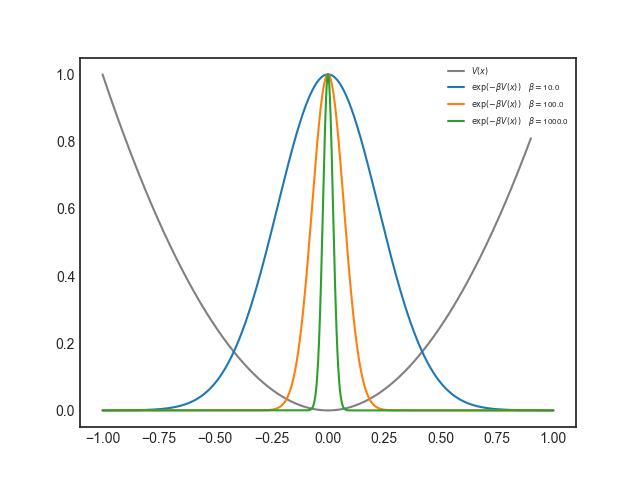
\includegraphics[width=0.9\textwidth]{Unnormalised_Gibbs_distribution.png}
\end{figure}
\end{frame}

\begin{frame}{Others}
\begin{enumerate}
    \item Maximum likelihood estimation
    \item Modelling \footnote{Skilling. The axioms of maximum entropy.}
    \item Clustering \footnote{Banerjee}
    \item Evolutionary algorithms
    \item Reinforcement learning \footnote{Hafner et al (2020). Action and perception as divergence minimisation.}
    \item Deep learning and backpropagation \footnote{Millidge, Tschantz and Buckley (2020). Predictive Coding Approximates Backprop along Arbitrary Computation Graphs.}
\end{enumerate}
\end{frame}


\begin{frame}{}
%\part{Some global theories of brain function}
\title{Part II: The second law of thermodynamics}
\author{\vspace{-5ex}}
\institute{\vspace{-5ex}}
\date{\vspace{-5ex}}
    \maketitle
    \small
\end{frame}

\begin{frame}{Setup}
\begin{itemize}
    \item Reach a target distribution known up to a normalisation constant.
    \item State-space: $\mathcal X$ a Polish space. e.g., separable, complete metric space.
\end{itemize}
\end{frame}

\begin{frame}{Markov processes}
\begin{itemize}
    \item A \textbf{stochastic process} $(X_t)_{t \geq 0}$ is a sequence of random variables $X_t$ on $\mathcal X$.
    \item A \textbf{Markov process} is a stochastic process such that the future is independent of the past, given the present.
\end{itemize}
\end{frame}

\begin{frame}{Diffusions and Markov jump processes}
    Def diffusion
    Def Markov jump process
    
    \begin{figure}
        \centering
        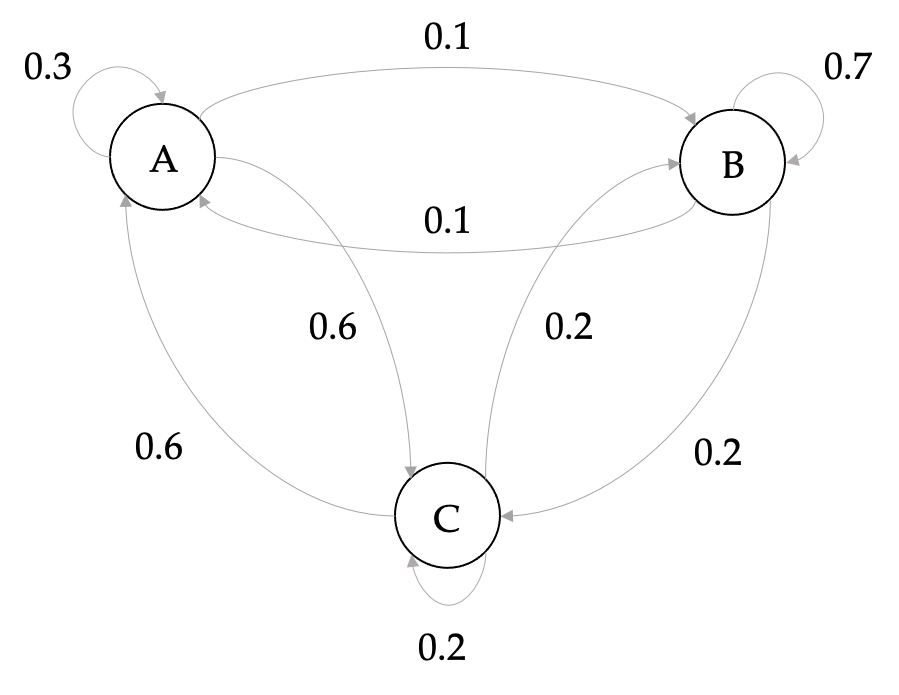
\includegraphics[width=0.7\textwidth]{Markov_chain.png}
    \end{figure}
\end{frame}

\begin{frame}{Markov semigroup, generator \& backward equation}
\begin{itemize}
    \item The \textit{semigroup} $\mathbf{P}_{t}$ tells us the evolution of observables (e.g., temperature, pressure etc)
    \begin{equation*}
    \mathbf{P}_{t}q(x) = \E [q(X_t)|X_0=x].
    \end{equation*}
    \item $\mathcal L$ is the \textit{generator} of the Markov process.
    \begin{equation*}
    \mathcal{L} q(x)= \lim_{\e \downarrow 0} \frac{\mathbf{P}_{\e} q(x) - q(x)}{\e}
    \end{equation*}
    \item $\mathbf{P}_{t}q$ solves the \textit{backward Kolmogorov equation}
    \begin{equation*}
        \partial_t q_{t}(x) = \mathcal L q_t(x).
    \end{equation*}
    %\item Given a reference distribution $p$ the backward Kolmogorov equation gives us a flow on the space of distributions
    %\begin{equation*}
    %    t \mapsto \mathbf{P}_{t}q p
    %\end{equation*}
\end{itemize}
\end{frame}

\begin{frame}{$(h, \Phi)$-entropies}
\begin{definition}[\footnote{M. L. Menendez, D. Morales, L. Pardo, and M. Salicru, (h-$\Phi$)- entropy differential metric, Appl. Math. 42-2 (1997), 81–98.}]
\begin{enumerate}
    \item $\Phi: \mathbb R \rightarrow \mathbb{R}$ smooth, convex.
    \item $h :\mathbb{R} \to \mathbb{R}$ arbitrary.
    \item $p$ a distribution.
\end{enumerate}
The $(h, \Phi)$-entropy of functions $g$ is defined as follows:
\begin{equation*}
    \H^{(h,\Phi)}[gp\mid p ]= \E_p[ \Phi ( g)] - h \circ \Phi \left(\E_p [ g ]\right).
\end{equation*}
\end{definition}
Examples:
\begin{enumerate}
    \item Variance: $ \operatorname{Var}_p[g]= \E_p[ g^2] -  \E_p [ g ]^2$
    \item $f$-divergences: $D_\Phi[g p \mid p ]$ %$h = 0  \Rightarrow  D_\Phi[g p \mid p ] = \E_p[\Phi(g)]$ 
    %\item $f$-divergences: $\Phi(1)=0 \Rightarrow D_\Phi[g p \mid p ] = \E_p[\Phi(g)]$
    \item KL divergence: $\dkl[g p \mid p]$.
    \item Reverse KL divergence: $\dkl[p \mid gp]$.
\end{enumerate}
\end{frame}

\begin{frame}{The second law of thermodynamics}
    \begin{theorem}
    Let $\left(X_{t}\right)_{t \geqslant 0}$ be a Markov process on a Polish space $\mathcal X$ and $p$ a steady-state. Let $\left(\mathbf{P}_{t}\right)_{t \geqslant 0}$ be the Markov semigroup with infinitesimal generator $\mathcal{L}$. Then, for any suitable function $g$: %Chafai also assumes t>0 and mu probability distribution, but it doesn't seem needed
    \begin{align*}
      \partial_{t} \H^{(h,\Phi)}[\mathbf{P}_t gp\mid p ]&=\E_{p}\left[\Phi^{\prime}\left(\mathbf{P}_{t} g\right) \mathcal {L} \mathbf{P}_{t} g\right] \leq 0.
    \end{align*}
\end{theorem}
\begin{itemize}
    \item[$\Rightarrow$] Given a target distribution $p$, the solution to the backward Kolmogorov equation $\mathbf{P}_t g p$ always gets closer to $p$.
\end{itemize}
\end{frame}



\begin{frame}{}
\title{Part III: The backward Kolmogorov equation as a gradient flow}
\author{\vspace{-5ex}}
\institute{\vspace{-5ex}}
\date{\vspace{-5ex}}
    \maketitle
    \small
\end{frame}

\begin{frame}{Gradient flows in metric spaces}
\begin{align*}
    -\nabla& F\\
    =&\\
    \text{"direction in which an infinitesimal}& \text{ increment in the \textbf{distance}}\\
    \text{leads to the largest decrease}& \text{ in the function"}
\end{align*}
\begin{figure}
    \centering
    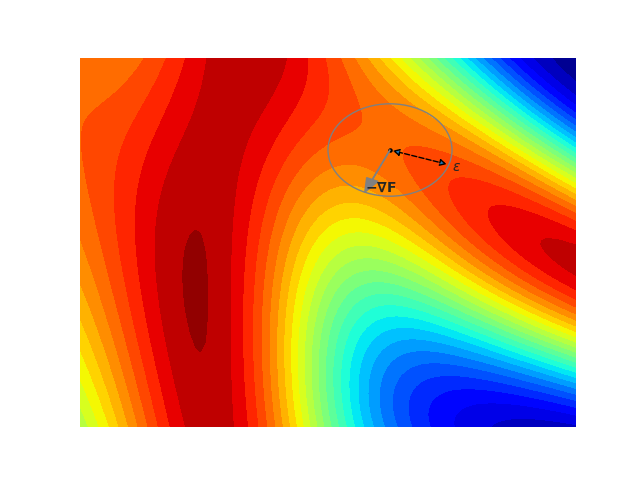
\includegraphics[width=0.49\textwidth]{Euclidean_gradient.png}
    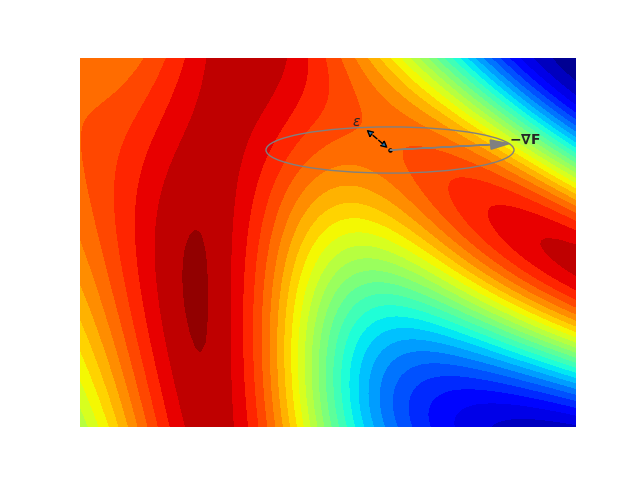
\includegraphics[width=0.49\textwidth]{Riemannian_gradient.png}
    \caption{Different metrics lead to different gradients.}
    \end{figure}
\end{frame}

\begin{frame}{Detailed balance}
    %Maybe slide last time
    Detailed balance = time-reversibility at steady-state.
    \vspace{10pt}
    
        TFAE for Markov processes at steady-state $p$\footnote{Jiang, Qian (2003). Mathematical theory of non-equilibrium steady-states.}
    \begin{itemize}
        \item $(X_t)_{t \geq 0}$ is time-reversible
        %\item The Markov process satisfies \textit{detailed balance},
        \item The entropy production rate vanishes,
                    $$e_p = \lim_{T\to \infty} \frac{1}{T}\dkl[\p_{[0,T]} \mid \p^-_{[0,T]} ]=0$$
        \item The generator $\mathcal L$ is symmetric in $L^2(p)$,
        $$ \int f \mathcal L g (x) \d p(x) = \int g \mathcal L f(x) \d p(x) \quad \forall f,g$$
    \end{itemize}
        \begin{figure}
        \centering
        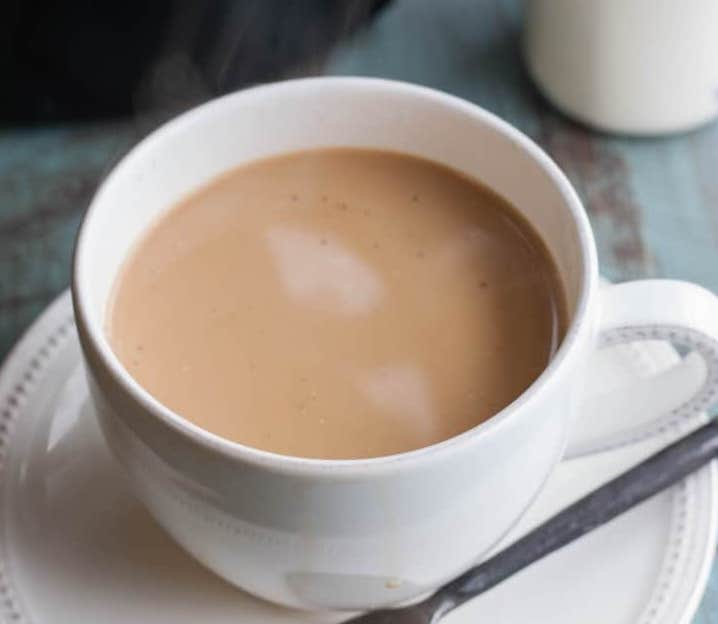
\includegraphics[width=0.3\textwidth]{coffee-cream-equilibrium.jpg}
        
\includegraphics[width=0.3\textwidth]{Coffee-cream-vortex.png}
    \end{figure}
\end{frame}

\begin{frame}{Markov jump processes}
        \begin{figure}
        \centering
        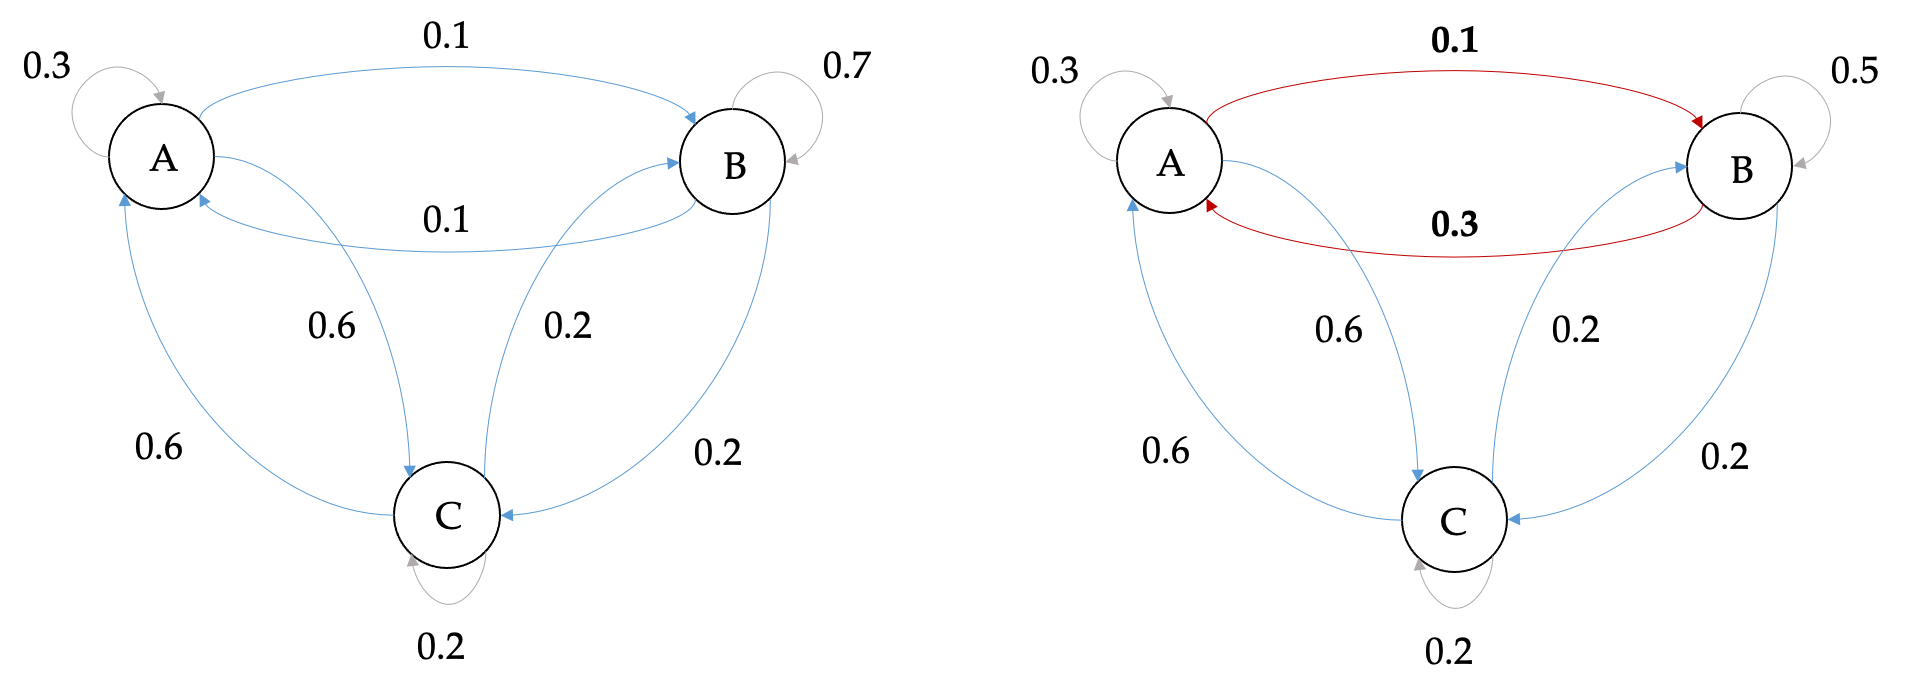
\includegraphics[width=0.8\textwidth]{MC_breaking_detailed_balance.png}
        \caption{Detailed balance (left), breaking detailed balance (right).}
        \end{figure}
        \begin{figure}
        \centering
        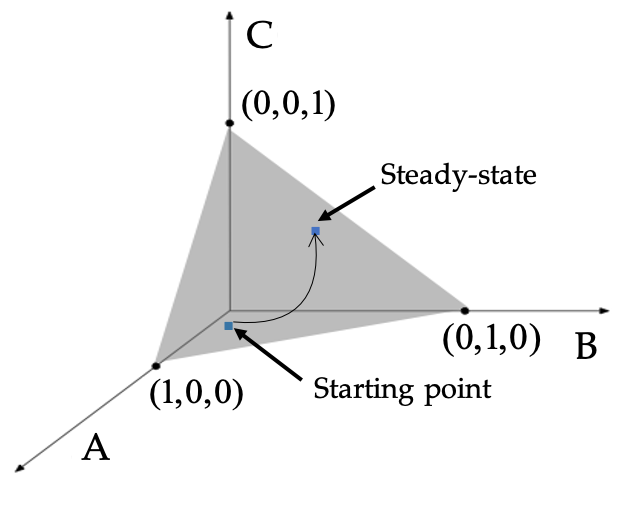
\includegraphics[width=0.4\textwidth]{Simplex_trajectory_MC.png}
        \caption{Dynamic on the space of probability distributions.}
        \end{figure}

\end{frame}

\begin{frame}{Markov jump processes}
\begin{theorem}[Maas, 2011 \footnote{J. Maas (2011). Gradient flows of the entropy for finite Markov chains.}]
Suppose the chain is irreducible and satisfies detailed balance with steady-state $p$.
\vspace{10pt}

The backward Kolmogorov equation is a gradient flow on $\dkl[\cdot \mid p]$ under an appropriate metric.
\end{theorem}
\end{frame}

\begin{frame}{Overdamped Langevin dynamics}
    \begin{equation*}
        \dot X_{t}=-\nabla V\left(X_{t}\right)+ \sqrt{2\beta^{-1}}\dot W_{t}
    \end{equation*}
    Has steady-state $p = Z^{-1}e^{-\beta V}$.
    
    \vspace{10pt}
    The Fokker-Planck equation
\begin{equation*}
\begin{split}
     \partial_t q_t &= \nabla \cdot \left(q_t \nabla \log \frac{q_t}{p}\right)\\
     &= \nabla \cdot \left(q_t \nabla \frac{\delta \dkl[q_t\mid p]}{\delta q_t}\right)
\end{split}
\end{equation*}
    is a gradient flow on 
    $$q \mapsto \dkl[q \mid p]$$
    under the Wasserstein metric.\footnote{Jordan, Kinderlehrer, Otto (1998). The variational formulation of the Fokker-Planck equation.}
\end{frame}

\begin{frame}{Reversible diffusions}
Any diffusion with a steady-state $p$ satisfying detailed balance is
\begin{align*}
    \dot X_{t}&=(\Sigma \nabla \log p+\nabla \cdot \Sigma)\left(X_{t}\right)+\sigma (X_t) \dot  W_{t}, \quad \Sigma := \frac{1}{2 }\sigma \sigma^T
\end{align*}
The Fokker-Planck equation is
\begin{equation*}
\begin{split}
     \partial_t q_t &= \nabla \cdot \left(q_t \Sigma \nabla \log \frac{q_t}{p}\right)\\
     &= \nabla \cdot \left(q_t \Sigma \nabla \frac{\delta \dkl[q_t\mid \rho]}{\delta q_t}\right)
\end{split}
\end{equation*}
Assume $\operatorname{det}\Sigma(x) >0, \forall x$. Then the FP equation is a gradient flow on
$$q \mapsto \dkl[q \mid p]$$
under the Kalman-Wasserstein metric\footnote{Garbuno-Inigo et al (2019). Interacting Langevin Diffusions- Gradient Structure And Ensemble Kalman Sampler.}
\end{frame}


\begin{frame}{}
\title{Part IV: Accelerating convergence}
\author{\vspace{-5ex}}
\institute{\vspace{-5ex}}
\date{\vspace{-5ex}}
    \maketitle
    \small
\end{frame}

\begin{frame}{A complete recipe for MCMC}
    Suppose we want to reach the distribution $\rho(x) \d x$ for smooth, positive $\rho$.
    
    Helmholtz decomposition: The complete set of diffusions that reaches the distribution $\rho$ is:
    
    We need to choose the one that converges the fastest.
\end{frame}

\begin{frame}{Irreversibility and hypoellipticity}
    %cup of coffee
    %Bellet 
    %Calculations Pavliotis
\end{frame}

\begin{frame}{State-of-the-art}
\begin{enumerate}
    \item Hamiltonian Monte-Carlo
    \item Particle methods: Stein variational inference
    \item Piecewise deterministic Markov processes \footnote{Bierkens et al (2016). The Zig-Zag Process and Super-Efficient Sampling for Bayesian Analysis of Big Data}
\end{enumerate}
\end{frame}

\begin{comment}
\begin{frame}{Overall summary}
    \begin{itemize}
        \item Reformulating many ML tasks in a common framework and applying well-known results in the mathematical community to solve them.
        \item The framework unifies a wide range of tasks and allows to compare, interpret and improve a wide range of algorithms.
    \end{itemize}
\end{frame}
\end{comment}


\begin{frame}
\title{Part V: Seeking advice}
\author{\vspace{-5ex}}
\institute{\vspace{-5ex}}
\date{\vspace{-5ex}}
    \maketitle
    \small
\end{frame}

\begin{frame}{Where to publish this?}
Currently $\approx$ 85 pages, 40500 words.
\begin{itemize}
    \item \textbf{SpringerBriefs}. Short book. 25000-52000 words.
    \item \textbf{JMLR}. ML audience. No word limit. Scope:
    \begin{itemize}
        \item Development of new analytical frameworks that advance theoretical studies of practical learning methods;
        %\item Theoretical studies yielding new insight into the design and behaviour of learning in intelligent systems;
        \item Surveys by invitation only.
    \end{itemize}
    \item \textbf{Entropy}. Interdisciplinary audience. No word limit.
\end{itemize}
\end{frame}


\begin{frame}{Thank you for listening}
\footnotesize
\vspace{10pt}
Special thanks to
\begin{multicols}{3}

    Supervisors\\
\vspace{10pt}
\textit{Greg Pavliotis\\
Karl Friston\\}
\vspace{10pt}
Collaborators\\
\vspace{10pt}
\textit{Alessandro Barp \\
Christopher Buckley\\
Danijar Hafner \\
Conor Heins \\
Casper Hesp\\
Beren Millidge\\
Sergio Rubin \\
Biswa Sengupta\\
Ryan Smith \\
Toby St Clere Smithe \\}
\vspace{10pt}
And colleagues \\
\vspace{10pt}
\textit{Victorita Neacsu \\
Thomas Parr\\
Benedikt Petko \\
Noor Sajid\\
Julian Sieber \\
Kai Ueltzhöffer \\
Sebastijan Veselic\\}
\end{multicols}
    \begin{figure}[ht]
    \centering
    
\includegraphics[width=.45\textwidth]{Figures/fnr_logo.png} \quad
    
\includegraphics[width=.45\textwidth]{Figures/cdtrandomsystemslogo.jpg} 
    \end{figure}
    \begin{figure}[ht]
    \centering
    
\includegraphics[width=.35\textwidth]{Figures/Imperial_college_logo.png}
    \quad
    
\includegraphics[width=.35\textwidth]{Figures/ucl-logo-colours-notext.png} 
    \end{figure}
\end{frame}
\end{document}